\documentclass{article}
\usepackage[margin=3cm]{geometry}
\usepackage{graphicx}
\usepackage{amsmath}
\usepackage{amsfonts}
\usepackage{physics}
\usepackage{float}

\title{DL HW2}
\author{Mehdi Jamalkhah}
\date{August 2024}

\newcommand*{\ex}[1]{
    \mathbb{E}_{#1}
}

\begin{document}

\maketitle

\section{Dropout vs. Batch Normalization}


\subsection{}
\begin{align*}
    \ex{D}[P]_{ij}
    = \ex{D}[(D \odot X)_{ij}] 
    = X_{ij} \ex{D}[D_{ij}]
    = X_{ij}((1 - p)(0) + p(1)) 
    = p X_{ij}
\end{align*}

\begin{align*}
    \ex{D}[(P^T P)]_{ij} =
    \begin{cases}
        \sum_{k=1}^{N} \ex{D}[D_{ki}D_{kj}X_{ki}X_{kj}]
        \overset{\text{$D_{ki}, D_{kj}$ are independent}}{=} 
        \sum_{k=1}^{N}\ex{D}[D_[ki]]\ex{D}[D_{kj}]X_{ki}X_{kj} \\
        \overset{\text{Bernoulli expectation is p}}{=} p^2 (X^TX)_{ij} &\text{if } i \neq j\\ \\
        \sum_{k=1}^{N} \ex{D}[D_{ki}^2X_{ki}X_{kj}] 
        = \sum_{k=1}^{N}\ex{D}[D_{ki}^2]X_{ki}X_{kj} 
        = ((p)(1^2) + (1 - p)(0^2)) (X^TX)_{ij} \\
        = p(X^TX)_{ij} &\text{if } i = j \\
    \end{cases}
\end{align*}


\subsection{}
\begin{align*}
    \ex{D}[||y - P\hat{w}||_2 ^ 2] 
    &= \ex{D}[(y - P\hat{w})^T (y - P\hat{w})] \\
    &= \ex{D}[(y^T - \hat{w}^T P^T)(y - P\hat{w})] \\
    &= \ex{D}[y^Ty - y^TP\hat{w} - \hat{w}^TP^Ty + \hat{w}^TP^TP\hat{w}] \\
    &= y^Ty - y^TpX\hat{w} - \hat{w}^T p X^T y + \hat{w}^Tp^2X^TX\hat{w} 
       + (-p^2 + P)\hat{w}^T\hat{\Gamma}^2\hat{w} \\
    &= (y^T - p\hat{w}^TX^T)(y - pX\hat{w}) + p(1 - p) \hat{w}^T\hat{\Gamma}^2\hat{w} \\
    &= ||y - pX\hat{w}||_2^2 + p(1 - p)||\hat{\Gamma}\hat{w}||_2^2
\end{align*}


\subsection{}
\begin{align*}
    w = p\hat{w} \Rightarrow
    &\ex{D}[||y - P\hat{w}||_2 ^ 2] \\
    &= ||y - Xw||_2^2 + \frac{1 - p}{p}||\hat{\Gamma}w||_2^2 \\
    &= ||y - Xw||_2^2 + ||\Gamma w||_2^2 \\
    &\Rightarrow \Gamma = \sqrt{\frac{1 - p}{p}} \hat{\Gamma}
\end{align*}


\subsection{}
\begin{align*}
    \Gamma w = \sqrt{\lambda}\tilde{w} &\Rightarrow w = \sqrt{\lambda} \Gamma^{-1} \tilde{w} \\
    \Rightarrow \mathbf{L}(\tilde{w}) 
    &= ||y - X\sqrt{\lambda} \Gamma^{-1} \tilde{w}||_2^2
    + \lambda ||\tilde{w}||_2^2 \\
    &= ||y-\tilde{X}\tilde{w}||_2^2 + \lambda ||\tilde{w}||_2^2 \quad ; \quad \tilde{X} = X\sqrt{\lambda} \Gamma^{-1}
\end{align*}

\begin{align*}
    \tilde{w}_i &= \alpha_i w_i \quad ; \quad \alpha_i = \lambda^{-0.5}\Gamma_{ii} \quad i = 1 \dots N \\
    \tilde{X}_{ij} &= \beta_j X_{ij} \quad ; \quad \beta_i = \lambda^{0.5}\Gamma_{ii}
\end{align*}


\subsection{}
As mentioned in the previous subsection, each element of the jth column 
of matrix X is divided by the jth element of the diagonal of gamma, which
is the sum of all elements in X multiplied by a constant. This means that
we are normalizing the batch.

In conclusion, using dropout is like to employing batch normalization with 
ridge regularization.


\subsection{}
\begin{align*}
    \pdv{J}{w_j} = (y_d - \sum_{k=1}^{n}(w_k + \delta_k)x_k)x_j \\
    \ex{\delta_k}[\pdv{J}{w_j}] = (y_d - \sum_{k=1}^{n}w_kx_k)x_j
\end{align*}


\subsection{}
\begin{align*}
    J 
    &= \frac{1}{2}(y_d - \sum_{k}(w_k - \delta_k)x_k)^2 \\
    &= \frac{1}{2}(y_d - sum_{k}w_kx_k + \sum_{k}\delta_kx_k)^2 \\
    &= \frac{1}{2}(y_d - sum_{k}w_kx_k)^2 + \frac{1}{2}(\sum_{k}\delta_kx_k)^2 + (\sum_k\delta_kx_k)(y_d - \sum_{k}w_kx_k) \\
    &= \frac{1}{2}(y_d - sum_{k}w_kx_k)^2 + \sum_{i}\sum_{j}\delta_i\delta_jx_ix_j +  (\sum_k\delta_kx_k)(y_d - \sum_{k}w_kx_k) \\
    &\Rightarrow \ex{\delta}[J] = \frac{1}{2}(y_d - \sum_{k}w_kx_k)^2 + \sum_{k} \alpha w_k^2x_k^2
\end{align*}

The final term resembles a regularization component, and it is a specific instance 
of Tikhonov regularization, where the $i$-th diagonal element is equal 
to $\sqrt{\alpha} x_i$.

\subsection{}
Spatial dropout sets an entire feature to zero, whereas this dropout technique 
makes some pixels zero. Consequently, the spatial filter will compel the model 
to not rely on a single filter, and the other force it to not depend on a specific
 pixel, which could correspond to a pattern in a particular image region.

In contrast, spatial dropout will lead to redundant features across different 
filters, while Gaussian dropout results in spatial redundancy.

\section{Backpropagation of CNN}
\begin{align*}
    \pdv{L}{W_j} = \sum_{i = 0}^{N - K + 1} \pdv{L}{Z_i} X_{i + j}
\end{align*}
This is the same as the convolution formula presented in formula 8, so we can 
derive the following formula:
\begin{align*}
    \pdv{L}{W} = \pdv{L}{Z} * X
\end{align*}



\section{Batch Normalization}

\subsection{}
\begin{align*}
    \pdv{L}{x} 
    &= \pdv{\hat{x}}{x} \pdv{y}{\hat{x}} \pdv{L}{y} 
    + \pdv{\sigma_B^2}{x}\pdv{\hat{x}}{\sigma_B^2}\pdv{y}{\hat{x}} \pdv{L}{y}
    + \pdv{\mu}{x} [ \pdv{\hat{x}}{\mu} + \pdv{\sigma_B^2}{\mu}\pdv{\hat{x}}{{\sigma_B^2}}] \pdv{y}{\hat{x}} \pdv{L}{y} \\
    &= \frac{1}{\sigma_B} \gamma \pdv{L}{y}
    + \frac{2}{m}(x - \mu_B)^T\frac{1}{\sigma_B} \gamma \pdv{L}{y}
    + \frac{-1}{m\sigma_B} \gamma[1 + \frac{2}{m}\sum_{i=1}^{m}(x_i - \mu_B)] \pdv{L}{y}
\end{align*}

\begin{align*}
    \pdv{L}{\gamma} = x^T \pdv{L}{y} \\
    \pdv{L}{\beta} = \sum_{i = 1}^{N} \pdv{L}{y_i}
\end{align*}


\subsection{}
\begin{enumerate}
    \item Improves gradient flow through the network; by reducing the dependence of gradients on the scale (or initialization) of the
    parameters
    \item Speedup the learning process because reduces the strong dependence on the initialization
    \item Acts as a form of regularization in a way that shown in first question.
\end{enumerate}


\subsection{}
Since we typically use batch normalization before the activation function 
(e.g., ReLU), if we do not properly locate the batch, half of the values will
be deleted, and this inactive bias will reduce the power of the model and may
not be consistent with the purpose of the model. Additionally, if we remove
the scale and shift, the output of all layers will become very similar,
and this will prevent progress in extracting good features from the data.


\subsection{}
Each batch is standardized in training time by subtracting its mean and dividing
 by its standard deviation. However, we perform the same calculation for test time 
 using the running average of the mean and standard deviation.

We expect to see approximately the same numbers during test time and train time,
which would happen if the data was well-shuffled. In this case, since each batch 
contains only a single class, the means can be very different from batch to batch.

As a result, the overall mean, which is more representative of the last batch, can 
be very different. It may be closer to the mean of class A, but we are testing a 
batch that contains class B, so the result is quite different from the train time.


\section{CNN Basic}
\subsection{}
No. Because this bais will be removed in shifting process of batch normalization.


\subsection{}
No. Because the output of convolution layer will scale to variance one in batch normalization.


\subsection{}
(i) \\
For each dot product: $k^2c$ \\
Number of dot products: $(\frac{w - k}{s} + 1)(\frac{h - k}{s} + 1)$ \\
Total: $k^2c(\frac{w - k}{s} + 1)(\frac{h - k}{s} + 1)$ \\
\\
\noindent
(ii) \\ 
For each pool average: $k^2c$ \\
Number of pool averages: $(\frac{w - k}{s} + 1)(\frac{h - k}{s} + 1)$ \\
Total: $k^2c(\frac{w - k}{s} + 1)(\frac{h - k}{s} + 1)$ \\
\\
\noindent
(iii) \\
Total: $whc$


\subsection{}
Reducing width of result tensor.(make more compacte features)


\subsection{}
Losing some information will lead to a more generalized model 
because it can not memorize all inputs.

\subsection{}
\begin{align*}
    \text{receptive field} = 2(2(\overbrace{2(\underbrace{1 \times 2}_{pool} - 1) + 3}^{conv}) - 1) + 3 = 21
\end{align*}



\section{MobileNet}


\subsection{}
\begin{figure}[H]
    \centering
    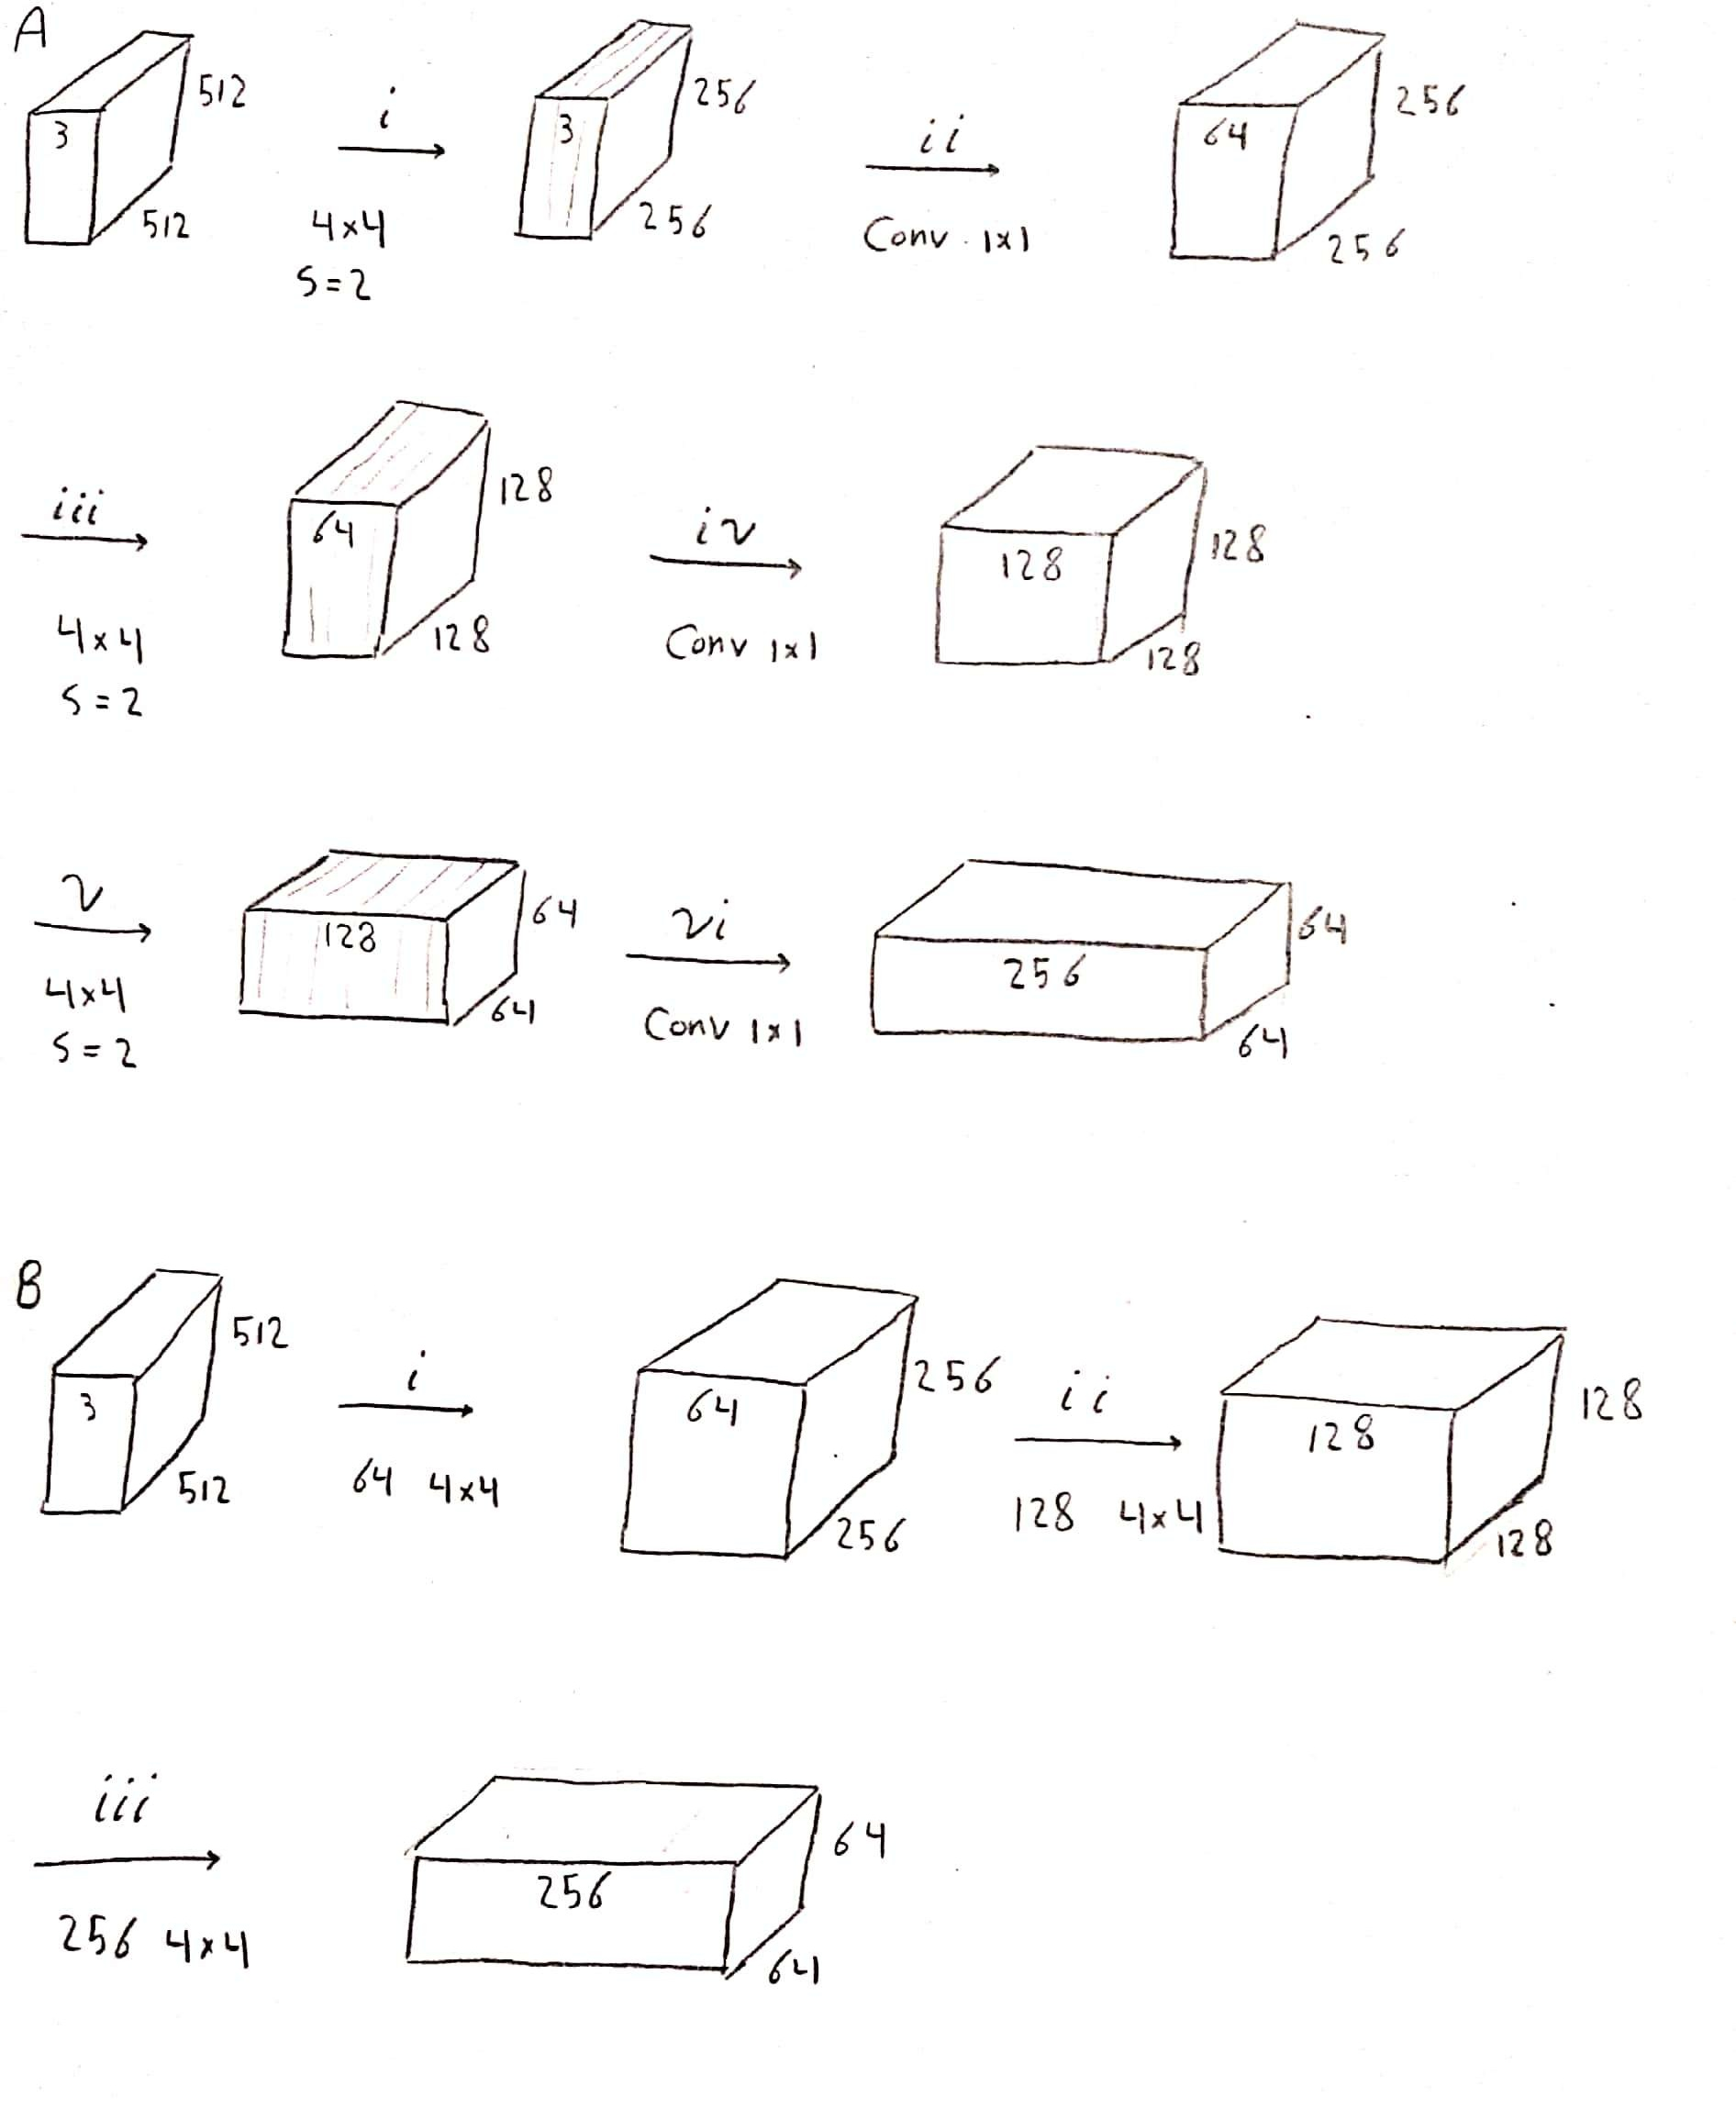
\includegraphics[width=0.5\linewidth]{figures/Q5_1.jpg}
    % \caption{}
    \label{fig:enter-label}
\end{figure}

\subsection{}
A:
\begin{align*}
    \#params = (3*4*4) + (64*3) + (64*4*4) + (128*64) + (128*4*4) + (128*256) = 44272
\end{align*}
\noindent
B:
\begin{align*}
    \#params = (64*3*4*4) + (128*64*4*4) + (256*128*4*4) = 658432
\end{align*}


\subsection{}
A:
\begin{align*}
    \# ops 
    &= (256*256*3*4*4) + (256*256*64*3) \\
    &+ (128*128*64*4*4) + (128*128*128*64) \\ 
    &+ (64*64*128*4*4) + (64*64*256*128) \\
    &= 309,329,920
\end{align*}

\noindent
B:
\begin{align*}
    \# ops
    &= (256*256*64*4*4*3) \\
    &+ (128*128*128*4*4*64) \\
    &+ (64*64*256*4*4*128) \\
    &= 4,496,293,888
\end{align*}


\subsection{}
Using depthwise separable convolutions compared to full convolutions for generating 
same size output is 15 times smaller and 14.5 times less compute intensive.

\subsection{}
The MobileNet model is based on depthwise separable convolutions which is a form of
factorized convolutions which factorize standard convolution into a depthwise 
convolution and a $1 \times 1$ convolution called pointwise convolution (As showed in 
previos sections). This factorization has the effect of drastically reducing compution and
model size.

Standard convolution have the computional cost of:
$$
    D_K \cdot D_k \cdot M \cdot N \cdot D_F \cdot D_F
$$
where the computional cost depends multiplicativeky on the number of input channels
$M$, the number of output channels $N$ the kernel size $D_k \times D_k$ and the 
feature map size $D_F \times D_F$. MobileNet uses depthwise separable convolutions to
break the interaction between the number of output channels and the size of the kernel.

Depthwise separable convolution cost is:
$$
    D_K \cdot D_K \cdot M \cdot D_F \cdot D_F + M \cdot N \cdot D_F \cdot D_F 
$$
which is the sum of the depthwise and $1 \times 1$ pointwise convolutions.
MobileNet get a reduction in computation of:
\begin{align*}
    \frac{D_K \cdot D_K \cdot M \cdot D_F \cdot D_F + M \cdot N \cdot D_F \cdot D_F }
    { D_K \cdot D_k \cdot M \cdot N \cdot D_F \cdot D_F}
    = \frac{1}{N} + \frac{1}{D_K^2}
\end{align*}
Result of expremints show that, for example, MobileNet is nearly as accurate as VGG16 while
being 32 times smaller and 27 times less compute intensive. It is more accurate than
GoogleNet while being smaller and more than 2.5 times less computation. 

In conclusion, it is not necessary to do two steps of standard convolution in one step
It is more efficient to only filters input channels, and then combine them
linearly to create new features.


\subsection{}
\begin{enumerate}
    \item \textbf{Width Multiplier: Thinner Models} \\
    In order to construct smaller and less computationally expensive models the 
    paper introduce a very simple parameter $\alpha$ called width multiplier. 
    For a given layer and width multiplier $\alpha$, the number of input channels 
    $M$ becomes $\alpha M$ and the number of output channels $N$ becomes $\alpha N$.
    where $\alpha in (0, 1])$. $\alpha = 1$ is the baseline MobileNet and $\alpha < 1$
    are reduced MobileNet. Width multiplier has the effect of reducing computional 
    cost and the number of parameters quadratically by roughly $\alpha^2$.

    \item \textbf{Resolution Multiplier: Reduced Representation} \\
    The second hyper-parameter to reduce the computional cost of a neural network is 
    resolution multiplier $\rho$. This multiplier will cahnge feature map size 
    $D_F \times D_F$ to $\rho D_F \times \rho D_F$. Resolution multiplier has the effect
    of reducing computational cost by $\rho^2$.
\end{enumerate}

Note that both parameters will reduce the accuracy for sake of less computional cost.



\section{Loss Function: Center Loss}

\subsection{}
In clustering, we should predict $y_i$, The loss function for this part of NN can be:
\begin{align*}
    y_i = \underset{k}{argmin} ||x_i - C_k||_2^2
\end{align*}
This loss function tries to find optimal class for a sample and center loss will make each class
more compact, means decreasing intra-class distance.

Actually this is same as k-means but we are in the space of deep features.


\subsection{}
\begin{align*}
    &x_i = W \hat{x_i} \\
    &\pdv{L}{x_i} = x_i - C_{y_i} \\
    &\pdv{L}{W} = \sum_{i = 1}^{m} \pdv{x_i}{W} \pdv{L}{x_i} 
    = \sum_{i = 1}^{m} (x_i - C_{y_i})\hat{x}_i^T \\
    &\pdv{L}{C_j} = C_{j} - \sum_{i: y_i = j}^{m}x_i
\end{align*}
\subsection{}
Center loss decrease the intra-class distance but do not Increasing the inter-class
distance This leads to misclassification. This paper make use of predefined evenly 
distribution class centroids, which makes the distance of inter-class be fixed and 
seprated from each other maximally.

The method of generating the predefined class center in the paper is based on the physical
model with the lowest isotropic charge energy on the sphere, that is, it is assumed that the charge
points on the hypersphere have repulsive force with each other, and the repulsive force decreases as
the distance between the points increases. At the end of the movement, the point on the hypersphere
stops moving. Due to the repulsive force, the points will be evenly distributed on the hypersphere.
When the equilibrium state is reached, the n points on the hypersphere can be farthest apart.
\end{document}

